\section{Stratified sampling by unstratified probability bounds}\label{section:old_statistics}




In this section we show how deriving (and subsequently minimising) inequalities such as these will allows for us to conduct stratified sampling in a single stage, rather than in two (as is nessisary in Neyman sampling).


But regardless of whether sampling is done with or without replacement, in the context of stratified sampling, inequalities such as EBBs cannot be directly minimised in quite the same way as Chebyschev's inequality can since the population mean itself does not have a sample variance, but only that the samples of the strata have means and sample variances.




However in this section, it is by these bounds that we can bind together EBB's of our choice to create a bound for the error of the stratified estimate - which we can then sample to minimise.

In this Section we develop a novel EBB derived from numerical computations, and compare it as a stratified sample mechanism against stratified sampling done with Maurer and Pontil's EBB and Audibert et.al's EBB, and also Neyman sampling in Chapter \ref{section:statistics_results}.

%We will also consider various EBBs in the context of Upper Confidence Bound (UCB) method of bandit algorithm in subsection \ref{}.

\subsection{Challenge: To derive a stronger EBB}

EBBs have been used as a method of generating confidence bounds for the mean, and an outstanding task is to see how much these techniques can be sharpened.
Given this challenge, we take inspiration and extend the work of \cite{Maurer50empiricalbernstein} to develop a new and stronger EBB.
Specifically, we use two Chernoff bounds, for the sample mean and the mean of sample squares, which are fused using a probability union (Theorem \ref{prob_union}) and variance decomposition (Theorem \ref{variance1}),
to create a novel probability bound for the sample variance, which is then used to derive our novel EBB.



%Our EBB tightens existing bounds by incorporating a combination of bounds on the variation of the sample variance.
%However, due to its analytic intractability, we complete the derivation by discussing how to numerically implement the bound.
%The evaluations in section \ref{} show that our EBB significantly tightens existing bounds. 
%Specifically, our EBB can shrink the best existing EBBs by about a third. This represents half of the distance between the best existing EBBs and an unattainable Bernstein bound constructed with perfect variance information.
%Moreover, we demonstrate the use of our novel EBB in an \textit{upper-confidence bound} (UCB) multi-armed bandit (MAB) algorithm in section \ref{}.  
%Results from a set of MABs show that using our bound in a UCB algorithm outperforms existing approaches, by producing comparable or lower expected regret than employing other existing bounds, including state-of-the-art EBBs.



% In addition, concentration inequalities that describe sampling without replacement can give additional tightening over those that assume sampling with replacement. This refinement was first demonstrated in \cite{serfling1974} with a martingale argument.
% More recently, this result was improved with a reverse martingale argument and used to extend M\&P's EBB to the case of sampling without replacement \cite{bardenet2015}.
% Furthermore, if small sample sizes are assumed, then it may be possible to derive perfectly tight %ideal 
% concentration inequalities in some circumstances, and there do exist some computational methods to derive these perfect bounds more generally \cite{OUQ1,doi:10.1137/13094712X}.
% However, in this paper we focus on refining bounds in the case of sampling with replacement in the context of large numbers of samples.


\subsubsection{Derivation and numerical implementation}
\label{derivation}
In this section, we derive two Chernoff bounds, 
for the sample mean and the mean of sample squares, (Theorem~\ref{sample_squares} and Lemma~\ref{variance2}, respectively). 
These are fused using a probability union and variance decomposition, defined above, to derive a bound for the sample variance. 
This bound is then used to derive our new EBB, as presented in Theorem~\ref{ebb1}.

Our first probability bound is a Chernoff bound on the sample mean called \textit{Bennett's inequality}. 
This bound is not new and was derived by \cite{hoeffding1} and \cite{10.2307/2282438} and has subsequently been a subject of discussion and many further developments; it is known to be quite strong \cite{Bentkus08boundsfor,Pinelis2014,zbMATH00812598}; 
We state the theorem \ref{hoeffdings1} whose proof involves the use of an intermediate theorem \ref{thm:parabola}.

\begin{theorem}[Bennett's inequality]\label{hoeffdings1}
Let $X$ be a real-valued random variable with a mean of zero and variance $\sigma^2$, that is bounded $a\le X\le b$. 
Then for $t>0$, the mean $\hat{\mu}$ of $n$ samples of $X$ is probability bounded by:
\begin{equation}\label{eq_no2}\p(\hat{\mu}\ge t)\le H_1^n\left(\frac{\sigma^2}{b^2},\frac{t}{b}\right),
\end{equation}
where:
\begin{equation*}
H_1^n\left(\frac{\sigma^2}{b^2},\frac{t}{b}\right) =
\left(\left(\frac{\frac{\sigma^2}{b^2}}{\frac{\sigma^2}{b^2}+\frac{t}{b}}\right)^{\frac{\sigma^2}{b^2}+\frac{t}{b}}
\left(1-\frac{t}{b}\right)^{\frac{t}{b}-1}\right)^{\frac{n}{\frac{\sigma^2}{b^2}+1}}
\end{equation*}
\end{theorem}
\begin{proof}As random variable X is bounded $a\le X\le b$, for any $s>0$, by Lemma \ref{thm:parabola}, there exist parameters $\alpha,\beta,\gamma$ such that, $\alpha s^2X^2+\beta sX+\gamma\ge \exp(sX)$ is always satisfied, hence for these we have:
$$\E\left[\exp(sX)\right] \le \E[\alpha s^2X^2+\beta sX+\gamma] \le \alpha s^2\E[X^2]+\gamma \le \alpha  s^2\sigma^2+\gamma$$
$$ \le (\sigma^2\exp(sb) + b^2\exp(-s\sigma^2/b))(\sigma^2 + b^2)^{-1}$$
Hence by application of lemma \ref{chernoff1}:\\
$$\p(\hat{\mu}\ge t) \;\le\; (\sigma^2\exp(sb) + b^2\exp(-s\sigma^2/b))^n((\sigma^2 + b^2)\exp(st))^{-n}$$
minimising with respect to $s$ completes the proof, minimum $s$ occurs at:
$$ s = \frac{b}{\sigma^2 + b^2}\log\left(\frac{b(\sigma^2 + tb)}{\sigma^2(b-t)}\right) $$
\end{proof}

\begin{lemma}[Parabola Fitting]\label{thm:parabola}
For $b>0$, $a<b$ and $z>0$, there exists an $\alpha,\beta,\gamma$ such that: $\alpha x^2+\beta x+\gamma\ge \exp(x)$ for all $a\le x\le b$, and:
$$z\alpha+\gamma = (z\exp(b) + b^2\exp(-z/b))(z + b^2)^{-1}$$
\end{lemma}
\begin{proof}
A example parabola $\alpha x^2+\beta x+\gamma$ which that satisfies these requirements tangentially touches the exponential curve at one point (at $x=f<b$) and intersects it at another (at $x=b$), as illustrated in Figure \ref{fig:graph1}.
Thus the parabola's intersection at $x=b$ and its tangential intersection at $x=f$ can be written in matrix algebra:
$$
\begin{bmatrix}
    \alpha \\
    \beta \\
	\gamma
\end{bmatrix}
=
\begin{bmatrix}
    b^2 & b & 1 \\
    f^2 & f & 1 \\
	2f  & 1 & 0
\end{bmatrix}^{-1}
\begin{bmatrix}
    \exp(b) \\
    \exp(f) \\
	\exp(f)
\end{bmatrix}$$
This gives our parabola parameters $\alpha,\beta,\gamma$, in terms of $f$ and $b$, hence:
$$z\alpha+\gamma = (((z+fb-b)(f-b-1)-b)e^f+(f^2+z)e^b)(b-f)^{-2}$$
Minimizing with respect to $f$ occurs at $f=\frac{-z}{b}$ and gives the result.
\end{proof}

The reason for the separation of Bennet's inequality into two parts is that we will reuse the Lemma to derive a weaker but more mathematically manipulatable inequality later (as Lemma \ref{expectation1}).
In our statement of Bennet's inequality the assumption that the mean is zero can be used without a loss of generality, in exactly the same way as we did with Hoeffding's inequality (Theorem \ref{Hoeffdings_inequality_proper}).
And so, Bennett's inequality gives us a probability bound for the difference of the sample mean from the true mean, given the variance - in a similar way as does Chebyshev's inequality.
The fundamental difference between Bennett's inequality and Hoeffding's inequality is the fitting of a parabola instead of a line over the exponential function.

As already stated, the variance is often unknown in practice, but can only be estimated via the sample variance statistic. And so we sought to derive a bound for the error between the sample variance and the variance. To do this we derived a concentration inequality for the sample squares to use in conjunction with the variance decomposition Lemma \ref{variance1}.
We derived the following concentration inequality (which we note, appears to be novel):

\begin{lemma}[Sample square bound]\label{sample_squares}
Let $X$ be a real-valued random variable with a mean of zero and variance $\sigma^2$, that is bounded $a\le X\le b$, if $d=\max(b,-a)$ then for $y>0$, the mean of sample squares $\hat{\sigma}_0^2=\frac{1}{n}\sum_ix_i^2$ is probability bounded:
\begin{equation}\label{equation_squares}\p(\sigma^2 - \hat{\sigma}_0^2> y) \le H_2^n\left(\frac{\sigma^2}{d^2},\frac{y}{d^2}\right),
\end{equation}
where:
\begin{align*} H_2^n\left(\frac{\sigma^2}{d^2},\frac{y}{d^2}\right) = \left(
\left(\frac{1-\frac{\sigma^2}{d^2}}{1+\frac{y}{d^2}-\frac{\sigma^2}{d^2}}\right)^{1+\frac{y}{d^2}-\frac{\sigma^2}{d^2}}
\left(\frac{\frac{\sigma^2}{d^2}}{\frac{\sigma^2}{d^2}-\frac{y}{d^2}}\right)^{\frac{\sigma^2}{d^2}-\frac{y}{d^2}}
\right)^n
\end{align*}
\end{lemma}

\begin{proof}
There exist parameters $\alpha,\gamma$ such for all $a\le X\le b$ that $\alpha X^2 + \gamma \ge \exp(-qX^2)$ whence:\\
$$\E[\exp(-qX^2)] \le \E[\alpha x^2 +\gamma] \le \alpha\sigma^2 + \gamma $$
With $d=\max(b,-a)$, we choose (see Fig \ref{fig:graph111}) $\alpha=(\exp(-qd^2)-1)d^{-2}$ and $\gamma=1$\\
Then applying lemma \ref{chernoff1} to the mean of the negated sample squares gives:\\
$$
\p(-\hat{\sigma}_0^2\ge t) \le \left(\frac{\sigma^2}{d^2}\exp(-qd^2)+1-\frac{\sigma^2}{d^2}\right)^n\exp(-qnt) 
$$
Substituting $t$ for $y-\sigma^2$ and minimizing with $q$ completes the proof, minimum $q$ occurs at:
$$ q = \frac{1}{d^2}\log\left(\frac{\sigma^2(-\sigma^2 + d^2 + y)}{(\sigma^2-d^2)(y-\sigma^2)}\right) $$
\end{proof}


It is worth noting that we choose to restrict the application of this inequality (and thence the domain of function $H_2^n$) to cases which are sensible for it to be applied:
(i) it is defined for $a<0<b$ (because otherwise the mean could not be zero), and (ii) $\sigma^2\le-ab\le (b-a)^2/4$ by Popoviciu's inequality (see \cite{zbMATH05780164}) as it is not possible for the variance to be larger given the width of the data bounds. It is important that we carried these domain restrictions with the analysis.

Since the Theorem \ref{sample_squares} is derived from a fundamentally similar process to Bennet's inequality we expect it to have similarly strong properties.


\begin{figure}[b]%
\centering
\parbox{2.5in}{

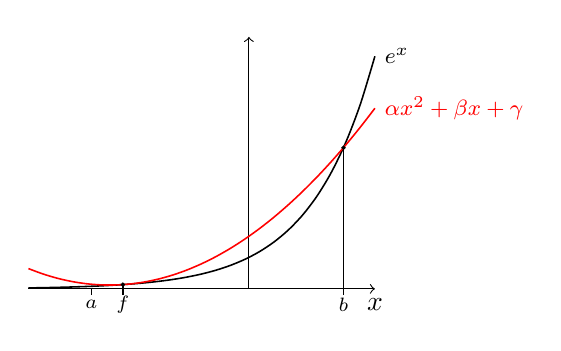
\begin{tikzpicture}[scale=0.8]
\draw[->] (-3.5,0) -- (2,0) node[anchor=north] {$x$};
\draw[->] (0,0) -- (0,4) node[anchor=east] {};
\draw[smooth, domain=-3.5:2.0, color=black, line width=0.20mm] 
    plot (\x,{e^(\x)/2}) node [right] {\footnotesize $e^x$};
\draw[smooth, domain=-3.5:2.0, color=red, line width=0.20mm] 
    plot (\x,{(0.316137167001903*\x*\x + 1.39988395124422*\x + 1.67055451771745)/2}) node [right] {\footnotesize $\alpha x^2+\beta x+\gamma$};
\draw (1.5,-0.1) -- (1.5,{e^(1.5)/2});
\draw (-2,-0.1) -- (-2,{e^(-2)/2});
\draw (-2.5,-0.1) -- (-2.5,0);
\draw[black,fill] (1.5,{e^(1.5)/2}) circle (0.25mm);
\draw[black,fill] (-2,{e^(-2)/2}) circle (0.25mm);
\draw	(-2.5,-0.25) node{{\scriptsize $a$}}
		(-2,-0.25) node{{\scriptsize $f$}}
		(1.5,-0.25) node{{\scriptsize $b$}};
\end{tikzpicture}

\caption[A parabola touching and intercepting an exponential curve]{A parabola parametarised by touching and intercepting points $f,b$ above an exponential curve for all $a\le x\le b$}%
\label{fig:graph1}}%
\qquad
\begin{minipage}{2.5in}%

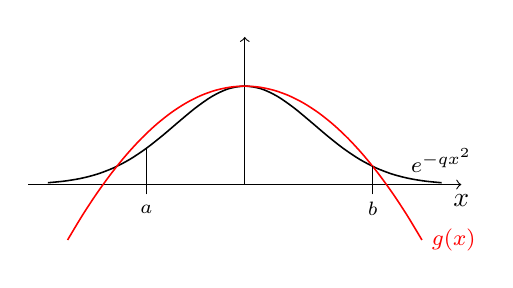
\begin{tikzpicture}[scale=1.25]
\draw[->] (-2.2,0) -- (2.2,0) node[anchor=north] {$x$};
\draw[->] (0,0) -- (0,1.5) node[anchor=east] {};
\draw[smooth, domain=-2.0:2.0, color=black, line width=0.20mm] 
    plot (\x,{e^(-(\x*\x))}) node [above] {\footnotesize $e^{-qx^2}$};
\draw[smooth, domain=-1.8:1.8, color=red, line width=0.20mm] 
    plot (\x,{-0.4825*\x*\x+1}) node [right] {\footnotesize $g(x)$};
\draw (1.3,-0.1) -- (1.3,{e^(-1.3*1.3)});
\draw (-1,-0.1) -- (-1,{e^(-1*1)});
\draw	(-1,-0.25) node{{\scriptsize $a$}}
		(1.3,-0.25) node{{\scriptsize $b$}};
\end{tikzpicture}

\caption[A parabola above a gaussian curve]{$g(x)=(e^{-qd^2}-1)d^{-2}x^2+1$ over function $f(x)=e^{-qx^2}$ for all $a\le x\le b$ where $d=\max(b,-a)$}%
\label{fig:graph111}%
\end{minipage}%
\end{figure}



At this point, we have a probability bound on the mean squared (Theorem \ref{hoeffdings1}) 
and a probability bound on the sample squares (Lemma \ref{sample_squares}). With these in hand, we use lemma \ref{variance1} to create a bound on the sample variance, as follows.


\begin{theorem}[Sample Variance Bound]\label{variance2}
For a random variable that is bounded $a\le X\le b$ with variance $\sigma^2$ and a mean of zero, if $d=\max(b,-a)$ then for $w>0$, the sample variance $\hat{\sigma}^2$ of $n$ samples is probability bounded by:
\begin{equation}\label{eq_no8}
\p(\sigma^2 - \hat{\sigma}^2 > w) \le H_3^n(a,b,w,\sigma^2),
\end{equation}
where:
\begin{align*} H_3^n(a,b,w,\sigma^2) =\min_{\phi\in[0,1]}
\begin{Bmatrix}
	H_1^n\left(\frac{\sigma^2}{b^2},\frac{\sqrt{\phi(\frac{n-1}{n}w+\frac{1}{n}\sigma^2)}}{b}\right)\\
	+H_1^n\left(\frac{\sigma^2}{a^2},\frac{-\sqrt{\phi(\frac{n-1}{n}w+\frac{1}{n}\sigma^2)}}{a}\right)\\
	+H_2^n\left(\frac{\sigma^2}{d^2},\frac{(1-\phi)(\frac{n-1}{n}w+\frac{1}{n}\sigma^2)}{d^2}\right)
\end{Bmatrix}\end{align*}
\end{theorem}
\begin{proof}By Lemmas \ref{sample_squares} and \ref{variance1}:
\begin{equation}\label{eq_no44}\p\left(\sigma^2 - \hat{\sigma}^2 > \frac{n}{n-1}\left(\hat{\mu}^2+y- \frac{1}{n}\sigma^2\right)\right) 
\le H_2^n\left(\frac{\sigma^2}{d^2},\frac{y}{d^2}\right)\end{equation}
By inspection of equation \ref{eq_no2} we can convert to a double-sided version:
\begin{equation}\label{eq_no1}\p(\hat{\mu}^2\ge r^2)= \p(\hat{\mu}\ge r)+\p(\hat{\mu}\le -r) \le H_1^n\left(\frac{\sigma^2}{b^2},\frac{r}{b}\right) + H_1^n\left(\frac{\sigma^2}{a^2},\frac{-r}{a}\right) \end{equation}
Also, by manipulating the inner inequality of this equation: \begin{equation}\label{eq_no33}\p\left(\frac{n}{n-1}\left(\hat{\mu}^2+y-\frac{1}{n}\sigma^2\right)\ge \frac{n}{n-1}\left(r^2+y-\frac{1}{n}\sigma^2\right)\right) \le H_1^n\left(\frac{\sigma^2}{b^2},\frac{r}{b}\right)+H_1^n\left(\frac{\sigma^2}{a^2},\frac{-r}{a}\right)\end{equation}
Applying lemma \ref{prob_union} to the equations \ref{eq_no33} and \ref{eq_no44} gives:
$$\p\left(\sigma^2 - \hat{\sigma}^2 > \frac{n}{n-1}\left(r^2+y-\frac{1}{n}\sigma^2\right)\right) \le H_2^n\left(\frac{\sigma^2}{d^2},\frac{y}{d^2}\right)+H_1^n\left(\frac{\sigma^2}{b^2},\frac{r}{b}\right)+H_1^n\left(\frac{\sigma^2}{a^2},\frac{-r}{a}\right)$$
For a choice of parameter $w=\frac{n}{n-1}\left(r^2+y-\frac{1}{n}\sigma^2\right)$ there is a range of possible $r,y>0$ which we can parameterise by value $\phi$, such that $0\le\phi\le 1$:
$$y(\phi) = (1-\phi)\left(\frac{n-1}{n}w+\frac{1}{n}\sigma^2\right) \quad\text{and}\quad
r(\phi)^2 = \phi\left(\frac{n-1}{n}w+\frac{1}{n}\sigma^2\right)$$
Thus:
$$\p\left(\sigma^2 - \hat{\sigma}^2 > w\right) 
\le H_2^n\left(\frac{\sigma^2}{d^2},\frac{y(\phi)}{d^2}\right) 
  + H_1^n\left(\frac{\sigma^2}{b^2},\frac{r(\phi)}{b}\right) + H_1^n\left(\frac{\sigma^2}{a^2},\frac{-r(\phi)}{a}\right)$$
The result of this proof follows by taking the minimum over $\phi$.
\end{proof}

The use of this Theorem \ref{variance2} (and thus implicitly the domain of function $H_3^n$) is subject to the same restrictions as Lemma \ref{sample_squares} (and its domain as $H_2^n$); specifically that it is defined for $a<0$ and $b>0$ and for $\sigma^2\le-ab$; as otherwise the configuration is senseless.

The development of this theorem for the bound of the error of the sample mean is derived from two strong concentration inequalities and a single probability union. The question then is how much that probability union manages to weaken the result.

Although the minimisation with $\phi$ is not very tractable, it can be conducted quickly for any situation on a computer via a parameter sweep.
Any lack of resolution on this sweep would not hamper the analytical accuracy of it as a bound - as an improper sweep could only be larger then what is possible.

To compare this bound against others, we cannot compare as-is, because we don't know $a$ and $b$ quite so much as we know that the data is bounded within a width of $D=b-a$.
To directly compare this bound against others we subsequently take the worst case $a,b$ consistent with a given $D$ and also $\sigma^2\le-ab$. And this process creates a bound which is directly comparable to other bounds such as Hoeffding's inequality among others.

From this action the resulting form of the bound is as follows:

\begin{theorem}[Sample Variance Bound]\label{variance22}
For a random variable that is bounded $a\le X\le b$ with variance $\sigma^2$, then for $w>0$, the sample variance $\hat{\sigma}^2$ of $n$ samples is probability bounded by:

\begin{equation}\label{eq_no9}
\p(\sigma^2 - \hat{\sigma}^2 > w) \le \max_{b\in[D/2,{D}/{2}+\sqrt{{D^2}/{4}-\sigma^2}]}\min_{\phi\in[0,1]}
\begin{Bmatrix}
	H_1^n\left(\frac{\sigma^2}{b^2},\frac{\sqrt{\phi(\frac{n-1}{n}w+\frac{1}{n}\sigma^2)}}{b}\right)\\
	+H_1^n\left(\frac{\sigma^2}{(b-D)^2},\frac{-\sqrt{\phi(\frac{n-1}{n}w+\frac{1}{n}\sigma^2)}}{b-D}\right)\\
	+H_2^n\left(\frac{\sigma^2}{\max(b,D-b)^2},\frac{(1-\phi)(\frac{n-1}{n}w+\frac{1}{n}\sigma^2)}{\max(b,D-b)^2}\right)
\end{Bmatrix}\end{equation}
\end{theorem}

The computational maximisation with respect to $b$ can also be done via parameter sweep.
Though this parameter sweep on $b$ may not necessarily respect analytical accuracy (since it is a maximisation, not a minimisation), we convert to this form only for the purposes of broad comparison with other bounds on the variance.

It is good to stop here to compare against other probability bounds for the error of the sample variance.
Particularly the bound on the variance developed by using Entropy method (as found in \cite{MR2245497} and used in \cite{Maurer50empiricalbernstein})

\begin{equation}\label{eq:fe} 
\p(\sigma^2 - \hat{\sigma}^2>w) \le \exp\left(\frac{-(n-1)w^2}{2\sigma^2D^2}\right) 
\end{equation}

And it is also possible to create a bound for the variance using the Efron-Stein method (\cite{efron1981}) with Chebyshev's inequality (for derivation see Appendix \ref{appendix:efron_chebyshev}), as:

\begin{equation}\label{eq:efron_stein_eq}\p\left(\sigma^2-\hat{\sigma}^2\ge k\right)\le\frac{5-n}{n(n-1)}\sigma^2 + \frac{D^4}{16nk^2}\end{equation}

And the strength of these bounds for the variance against our bound can be graphically compared as per Figure \ref{fig:variance_graph1}.
From this graph we see that our bound performs better at creating lighter tail bounds for the sample variance estimator but that different methods work better-or-worse in different regions - as divergent methods produce differing results.\footnote{We do however note that the graph ouf our variance bound on this figure was produced after taking the worst case $a,b$ consistent with a $D=1$, and the manner in which we use it subsequently avoids this deterioration, until a later stage.}


    \begin{figure}[]
        \centering
		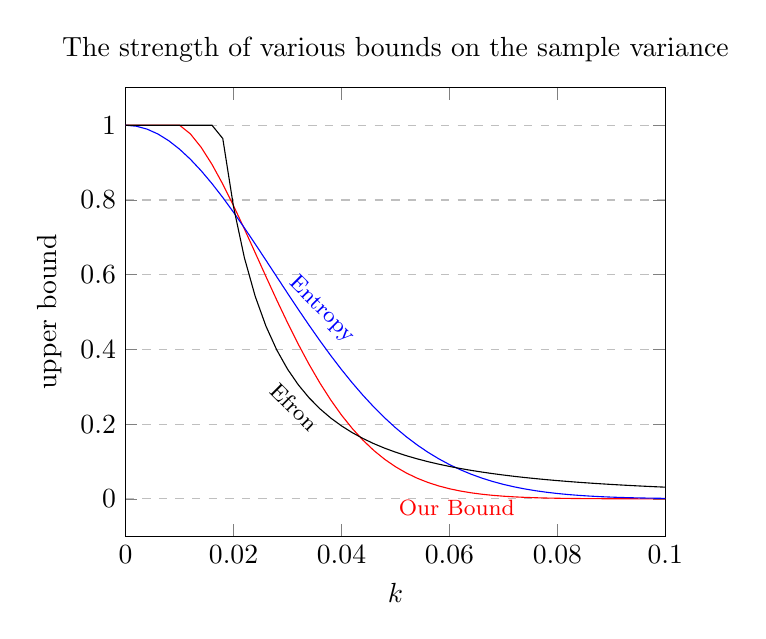
\begin{tikzpicture}
		\begin{axis}[
			title={The strength of various bounds on the sample variance},
			xlabel={$k$},
			ylabel={upper bound},
			xmin=0, xmax=0.1,
			%ymin=0.001, ymax=0.05,
			%ymode=log,
			%xtick={0,0.05,0.1,0.15,0.2,0.25},
			%ytick={0,20,40,60,80,100},
			%yticklabel=$\pgfmathprintnumber{\tick}\%$,
			legend pos=south west,
			ymajorgrids=true,
			grid style=dashed,
			xticklabel style={/pgf/number format/fixed}
		]
		\addplot[color={rgb:red,1;green,0;yellow,0}] coordinates {
(0.000000, 1.000000)(0.002000, 1.000000)(0.004000, 1.000000)(0.006000, 1.000000)(0.008000, 1.000000)(0.010000, 1.000000)(0.012000, 0.976796)(0.014000, 0.940761)(0.016000, 0.895277)(0.018000, 0.842473)(0.020000, 0.784293)(0.022000, 0.722562)(0.024000, 0.658973)(0.026000, 0.595056)(0.028000, 0.532153)(0.030000, 0.471397)(0.032000, 0.413695)(0.034000, 0.359740)(0.036000, 0.310013)(0.038000, 0.264798)(0.040000, 0.224211)(0.042000, 0.188221)(0.044000, 0.156675)(0.046000, 0.129339)(0.048000, 0.105899)(0.050000, 0.086012)(0.052000, 0.069309)(0.054000, 0.055417)(0.056000, 0.043973)(0.058000, 0.034631)(0.060000, 0.027074)(0.062000, 0.021015)(0.064000, 0.016197)(0.066000, 0.012397)(0.068000, 0.009425)(0.070000, 0.007118)(0.072000, 0.005341)(0.074000, 0.003983)(0.076000, 0.002951)(0.078000, 0.002173)(0.080000, 0.001591)(0.082000, 0.001158)(0.084000, 0.000838)(0.086000, 0.000603)(0.088000, 0.000431)(0.090000, 0.000307)(0.092000, 0.000217)(0.094000, 0.000153)(0.096000, 0.000107)(0.098000, 0.000074)(0.100000, 0.000052)(0.102000, 0.000035)(0.104000, 0.000024)(0.106000, 0.000017)(0.108000, 0.000011)(0.110000, 0.000008)(0.112000, 0.000005)(0.114000, 0.000003)(0.116000, 0.000002)(0.118000, 0.000001)(0.120000, 0.000001)(0.122000, 0.000001)(0.124000, 0.000000)(0.126000, 0.000000)(0.128000, 0.000000)(0.130000, 0.000000)(0.132000, 0.000000)(0.134000, 0.000000)(0.136000, 0.000000)(0.138000, 0.000000)(0.140000, 0.000000)(0.142000, 0.000000)(0.144000, 0.000000)(0.146000, 0.000000)(0.148000, 0.000000)
        }node[pos=0.91](endofplotsquare){} ;
		\node [below,color={rgb:red,1;green,0;yellow,0}] at (endofplotsquare) {\footnotesize Our Bound};
		\addplot[color={rgb:red,0;blue,1;yellow,0}] coordinates {
(0, 1.0) (0.002, 0.997350183644) (0.004, 0.989442789364) (0.006, 0.976402871073) (0.008, 0.958435191453) (0.01, 0.935818872672) (0.012, 0.908900183468) (0.014, 0.87808372306) (0.016, 0.843822315395) (0.018, 0.806605966074) (0.02, 0.766950257277) (0.022, 0.725384562782) (0.024, 0.682440455785) (0.026, 0.638640657998) (0.028, 0.594488841053) (0.03, 0.550460543126) (0.032, 0.506995407644) (0.034, 0.464490890034) (0.036, 0.423297515852) (0.038, 0.383715712221) (0.04, 0.345994177074) (0.042, 0.310329699467) (0.044, 0.276868301049) (0.046, 0.245707534782) (0.048, 0.216899752983) (0.05, 0.19045614263) (0.052, 0.166351321354) (0.054, 0.144528291741) (0.056, 0.124903563263) (0.058, 0.107372268989) (0.06, 0.0918131266269) (0.062, 0.0780931188187) (0.064, 0.0660717944596) (0.066, 0.0556051197572) (0.068, 0.0465488335613) (0.07, 0.0387612852497) (0.072, 0.0321057544037) (0.074, 0.0264522691726) (0.076, 0.0216789543788) (0.078, 0.0176729510065) (0.08, 0.0143309558975) (0.082, 0.0115594345264) (0.084, 0.00927456102917) (0.086, 0.00740193865015) (0.088, 0.00587615094073) (0.09, 0.00464018983902) (0.092, 0.00364480164518) (0.094, 0.0028477862716) (0.096, 0.00221327933787) (0.098, 0.0017110409802) (0.1, 0.0013157698685) (0.102, 0.00100645602988) (0.104, 0.00076578176314) (0.106, 0.000579576245108) (0.108, 0.000436326387277) (0.11, 0.000326744076771) (0.112, 0.00024338808442) (0.114, 0.000180337583441) (0.116, 0.000132913325077) (0.118, 9.74419898103e-05) (0.12, 7.10590028484e-05) (0.122, 5.15451037129e-05) (0.124, 3.71921316689e-05) (0.126, 2.6693779426e-05) (0.128, 1.90574332941e-05) (0.13, 1.35336235817e-05) (0.132, 9.56002706345e-06) (0.134, 6.71737346447e-06) (0.136, 4.6949958307e-06) (0.138, 3.26412116474e-06) (0.14, 2.25731764273e-06) (0.142, 1.55279607415e-06) (0.144, 1.06250630718e-06) (0.146, 7.23175913889e-07) (0.148, 4.89611639113e-07)
        }node[pos=0.5](endofplotsquare){} ;
		\node [above,color={rgb:red,0;blue,1;yellow,0}, rotate=-45] at (endofplotsquare) {\footnotesize Entropy};
		\addplot[black] coordinates {
(0, 1) (0.002, 1.0) (0.004, 1.0) (0.006, 1.0) (0.008, 1.0) (0.01, 1.0) (0.012, 1.0) (0.014, 1.0) (0.016, 1.0) (0.018, 0.96450617284) (0.02, 0.78125) (0.022, 0.645661157025) (0.024, 0.542534722222) (0.026, 0.462278106509) (0.028, 0.398596938776) (0.03, 0.347222222222) (0.032, 0.30517578125) (0.034, 0.270328719723) (0.036, 0.24112654321) (0.038, 0.216412742382) (0.04, 0.1953125) (0.042, 0.177154195011) (0.044, 0.161415289256) (0.046, 0.147684310019) (0.048, 0.135633680556) (0.05, 0.125) (0.052, 0.115569526627) (0.054, 0.107167352538) (0.056, 0.0996492346939) (0.058, 0.0928953626635) (0.06, 0.0868055555556) (0.062, 0.0812955254943) (0.064, 0.0762939453125) (0.066, 0.0717401285583) (0.068, 0.0675821799308) (0.07, 0.0637755102041) (0.072, 0.0602816358025) (0.074, 0.0570672023375) (0.076, 0.0541031855956) (0.078, 0.0513642340565) (0.08, 0.048828125) (0.082, 0.0464753123141) (0.084, 0.0442885487528) (0.086, 0.0422525689562) (0.088, 0.040353822314) (0.09, 0.0385802469136) (0.092, 0.0369210775047) (0.094, 0.0353666817565) (0.096, 0.0339084201389) (0.098, 0.0325385256143) (0.1, 0.03125) (0.102, 0.0300365244137) (0.104, 0.0288923816568) (0.106, 0.0278123887504) (0.108, 0.0267918381344) (0.11, 0.025826446281) (0.112, 0.0249123086735) (0.114, 0.0240458602647) (0.116, 0.0232238406659) (0.118, 0.02244326343) (0.12, 0.0217013888889) (0.122, 0.0209957000806) (0.124, 0.0203238813736) (0.126, 0.0196837994457) (0.128, 0.0190734863281) (0.13, 0.0184911242604) (0.132, 0.0179350321396) (0.134, 0.0174036533749) (0.136, 0.0168955449827) (0.138, 0.0164093677799) (0.14, 0.015943877551) (0.142, 0.0154979170799) (0.144, 0.0150704089506) (0.146, 0.0146603490336) (0.148, 0.0142668005844)
        }node[pos=0.7](endofplotsquare){} ;
		\node [below,black, rotate=-45] at (endofplotsquare) {\footnotesize Efron};
		
		\end{axis}
		\end{tikzpicture}
		%\vspace{-18pt}
		\caption{The upper bound on $ \p(\sigma^2-\hat{\sigma}^2\ge k) $ for various $k$, at $\sigma^2=0.1$ for $D=1, n=200$ using the Entropy method (Equation \ref{eq:fe}), the Efron-Stein method (Equation \ref{eq:efron_stein_eq}), and our method (via Theorem \ref{variance2})}
		\label{fig:variance_graph1}
    \end{figure}



Because of this plurality, it is always possible to use the minima of several different variance bounds together, so in constructing our EBB, we took the minima of all three.


And so by Theorem \ref{hoeffdings1}, we have a bound for the sample mean given the variance, and in Theorem \ref{variance2} we have a probability bound for the error of the sample variance from the variance (in conjunction with the minima of the other two bounds on the variance). The task to create a new Empirical Bernstein Bound is bind these two together.

We used a method of combining these two to create a bound for the sample mean given the sample variance, by a theorem that embodies a process slightly improved from that followed by \cite{Maurer50empiricalbernstein}. 

Before beginning this theorem, we need to introduce some notation.
For a function $f$ with ordered inputs, we denote the inverse of $f$ with respect to its $i${th} input (counting from one) as $f^{-(i)}$, assuming it exists.
We summarily denote probability bounds on the differences of the sample mean from the mean, and the sample variance from the variance, by
$\p(\hat{\mu}-\mu>t)\le h(\sigma^2,t)$ and $\p(\sigma^2-\hat{\sigma}^2>w)\le f(\sigma^2,w)$, respectively.
And note that functions $h$ and $f$ may have additional arguments not limited to $\sigma^2$ and $t$, and $\sigma^2$ and $w$, respectively; but that these are not considered in the theorem and proof for brevity.

\begin{theorem}[Essential EBB]\label{ebb1} 
Assume $f^{-(2)}$ and $h^{-(2)}$ both exist, and also if $h^{-(2)}$ is monotonically increasing in its first argument, so that we can define:
\[
z(\sigma^2,w) = \sigma^2-f^{-(2)}\left(\sigma^2,w\right)
\]
If $z^{-(1)}$ exists and is monotonic increasing in its first argument, then for any $x\in[0,y]$, the following relationship holds:
\[
\p\left(\hat{\mu}-\mu>h^{-(2)}\left(z^{-(1)}\left(\hat{\sigma}^2,y-x\right),x\right)\right)
\le y
\]
\end{theorem}
%
\begin{proof}
Substituting $w$ for $f^{-2}(\sigma^2,w)$ gives:
%$\p(\sigma^2-\hat{\sigma}^2>f^{-2}(\sigma^2,w))\le w$\\
%$\p(z(\sigma^2,w)>\hat{\sigma}^2)\le w$\\
%$\p(\sigma^2>z^{-1}(\hat{\sigma}^2,w))\le w$\\
%$\p(h^{-2}(\sigma^2,t)>h^{-2}(z^{-1}(\hat{\sigma}^2,w),t))\le w$\\
\begin{align*}
w & \ge \p\left(\sigma^2-\hat{\sigma}^2>f^{-(2)}\left(\sigma^2,w\right)\right)\\
 & \ge \p\left(z\left(\sigma^2,w\right)>\hat{\sigma}^2\right)\\
 & \ge \p\left(\sigma^2>z^{-(1)}\left(\hat{\sigma}^2,w\right)\right)\\
 & \ge \p\left(h^{-2}\left(\sigma^2,t\right)>h^{-(2)}\left(z^{-(1)}\left(\hat{\sigma}^2,w\right),t\right)\right)
\end{align*}
% $w  \ge \p(\sigma^2-\hat{\sigma}^2>f^{-2}(\sigma^2,w))$\\
% \-\hspace{4mm}$\ge \p(z(\sigma^2,w)>\hat{\sigma}^2)$\\
% \-\hspace{4mm}$\ge \p(\sigma^2>z^{-1}(\hat{\sigma}^2,w))$\\
% \-\hspace{4mm}$\ge \p(h^{-2}(\sigma^2,t)>h^{-2}(z^{-1}(\hat{\sigma}^2,w),t))$\\
Substituting $t$ for $h^{-(2)}(\sigma^2,t)$ gives:
\[
\p\left(\hat{\mu}-\mu>h^{-(2)}\left(\sigma^2,t\right)\right)
\le t.
\]
Applying probability union (lemma \ref{prob_union}) gives:\\
\[
\p\left(\hat{\mu}-\mu>h^{-(2)}\left(z^{-(1)}\left(\hat{\sigma}^2,w\right),t\right)\right)
\le t+w.
\]
Letting $y=t+w$ and $x=y-w$ completes the proof.
\end{proof}

The result of this Theorem is an Empricial Bernstein Bound. And our novel EBB is completed by substituting  $h(\sigma^2,t)=H_1^n\left(\sigma^2/b^2,t/b\right)$ (from Theorem \ref{hoeffdings1}) and $f(\sigma^2,w)=H_3^n\left(a,b,w,\sigma^2\right)$ (from Theorem \ref{variance2}) into Theorem \ref{ebb1}.
In this process care was taken in applying this theorem that all the assumptions hold, the necessary inverses exist, and that the domains of the functions were propagated through the analysis.




\subsubsection{Numerical implementation}
\label{numerical-implementation}
Analytically solving this our EBB was challenging, however it was possible to evaluate it to arbitrary accuracy using numerical techniques.
This section provides a high-level description of a process that was used for calculating our EBB.

This calculation was composed of three primary parts:
(i) the computation of function $f(\sigma^2,w)=H_3^n(a,b,y,\sigma^2)$;
(ii) verifying that the assumptions of Theorem \ref{ebb1} hold for $h(\sigma^2,t)=H_1$ and $f(\sigma^2,w)=H_3$, and;
(iii) calculating the subsequent result of Theorem \ref{ebb1}.

First, the function $f(\sigma^2,w)=H_3^n(a,b,w,\sigma^2)$ (per Theorem \ref{variance2}) is the solution to an optimization problem that solves for the minima of an objective function subject to constraint $\phi\in[0,1]$.
Despite its complexity, a solution can be found quickly using a single variable parameter sweep.

Second, it was necessary to verify the assumptions that $h^{-(2)}$, $f^{-(2)}$ and $z^{-(1)}$ exist and that $z^{-(1)}$ and $f^{-(2)}$ are monotonically increasing in their first argument.
It was easy to note that $h(\sigma^2,t)=H_1^n\left(\sigma^2/b^2,t/b\right)$ is a closed-form function that is monotonically decreasing from $1$ to $0$ on the second argument, so $h^{-(2)}$ exists and is monotonically increasing in its first argument.  However the remaining of these assumptions are more difficult to verify.
For any function, the values that the function takes can be plotted as an array of points and the values that the inverse of that function takes can be determined by conducting coordinate swaping on those points.
The values of $f(\sigma^2,w)=H_3^n(a,b,w,\sigma^2)$ were computed and were seen to be monotonically decreasing in its second argument confirming that $f^{-(2)}$ exists.
The function $z(\sigma^2,w)=\sigma^2-f^{-(2)}\left(\sigma^2,w\right)$ is then a manipulation on the coordinate swapped points of $f(\sigma^2,w)=H_3^n(a,b,w,\sigma^2)$.
By coordinate swapping again, $z^{-(1)}$ was seen to be a regular function monotonically increasing on its first argument, hence satisfying assumptions.


Third, to numerically calculate the result of Theorem \ref{ebb1} the functions $h^{-(2)}$ and $z^{-(1)}$ were numerically evaluated by direct parameter searches and then composed as:
$h^{-(2)}(z^{-(1)}(\hat{\sigma}^2,y-x),x)$ - which was the inner part of the expression of the new EBB parameterised by $x$ explicitly and also $a,b$ implicitly.
%
However we typically don't know the values of $a$ and $b$, but instead know the mean is somewhere within a finite interval of width $D=b-a$.
So in a similar way as was handled by introduction of Theorem \ref{variance22}, we took the worst case values of $a$ and $b$ consistent with a given $D$, 
and then took the best $x\in[0,y]$ subject to all other bounds.
In short, the numerical process involved a series of coordinate manipulations to conduct inversions and some mundane parameter searches.\footnote{sourcecode available at:\\\url{https://github.com/Markopolo141/Engineered-Empirical-Bernstein-Bound}}

\subsection{Comparison to existing bounds}\label{evaluation}
By being able to numerically evaluate our EBB, we were able to compare the strength of our results against existing concentration bounds, particularly our EBB is compared to Maurer and Pontil's EBB and, Bennett's inequality with perfect variance information.

We compared our EBB directly with \cite{Maurer50empiricalbernstein}'s EBB, 
given by:
\begin{equation}\label{maurersbound} \p\left(\mu-\hat{\mu}>\sqrt{\frac{2\hat{\sigma}^2\log(2/y)}{n}}+\frac{7D\log(2/y)}{3(n-1)}\right)<y. \end{equation}
We felt that it would be fair to compare our EBB to Maurer and Pontil's EBB if they had applied Popoviciu's inequality as a domain restriction and carried it through their derivation, as we did to our own EBB. 
Specifically, this is the domain where:
\[ \frac{1}{2}>\frac{\sqrt{\hat{\sigma}^2}}{D}+\sqrt{\frac{2\log(2/y)}{n-1}} \]
We plotted the improvement our EBB offers in this domain, as shown in Figure \ref{biggraph3}. 
In this plot, a probability 0.5 bound is shown to shrink by approximately one third.
But that generally, we observed that our refinement of Maurer and Pontil's EBB was expectedly uniformly tighter across a large range of values.



\begin{figure}[]{}
    \centering
	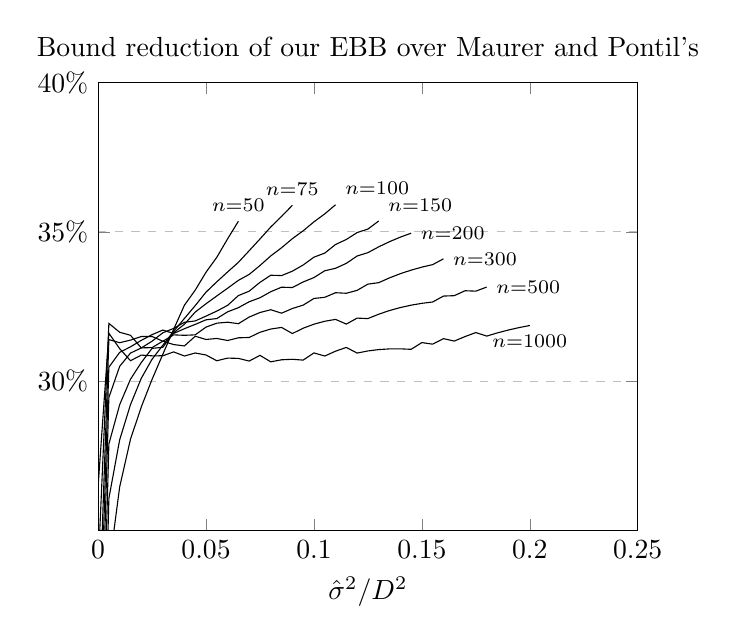
\begin{tikzpicture}
	\begin{axis}[
		title={Bound reduction of our EBB over  Maurer and Pontil's},
		xlabel={$\hat{\sigma}^2/D^2$},
		xmin=0, xmax=0.25,
		ymin=25, ymax=40,
		xtick={0,0.05,0.1,0.15,0.2,0.25},
		ytick={30,35,40},
		yticklabel=$\pgfmathprintnumber{\tick}\%$,
		ymajorgrids=true,
		grid style=dashed,
		xticklabel style={/pgf/number format/fixed},
	]
	\addplot[] coordinates {
(0.0, 10.038489469957923)(0.005, 23.729228874038338)(0.01, 26.46795119155083)(0.015, 28.061119743643296)(0.02, 29.141938583623652)(0.025, 30.066155991693723)(0.03, 30.907282335052788)(0.035, 31.738722848538305)(0.04, 32.54914392836502)(0.045, 33.05291848928947)(0.05, 33.651509619741496)(0.055, 34.151805087746446)(0.06, 34.768247610158575)(0.065, 35.35764746719292)
		}node[pos=1.0](endofplotsquare){} ;
	\node [above] at (endofplotsquare) {$\scriptstyle n=50$};
	\addplot[] coordinates {
(0.0, 12.591458904845746)(0.005, 26.08582516018055)(0.01, 28.044488963240152)(0.015, 29.219014176778845)(0.02, 30.101019545112305)(0.025, 30.739739304373572)(0.03, 31.209391146592484)(0.035, 31.67459564986504)(0.04, 32.10560417423678)(0.045, 32.53522214247566)(0.05, 32.98480753922602)(0.055, 33.33123349968554)(0.06, 33.66064263107598)(0.065, 33.983296057116895)(0.07, 34.371432119724126)(0.075, 34.76400092304011)(0.08, 35.165771922230526)(0.085, 35.51929445366766)(0.09, 35.890640326573575)
		}node[pos=1.0](endofplotsquare){} ;
	\node [above] at (endofplotsquare) {$\scriptstyle n=75$};
	\addplot[] coordinates {
(0.0, 14.817995440815901)(0.005, 27.90751007185735)(0.01, 29.219819451516923)(0.015, 30.070639062533996)(0.02, 30.629290720122317)(0.025, 31.104197838170627)(0.03, 31.14038996461402)(0.035, 31.62526607199946)(0.04, 31.911575841232846)(0.045, 32.3187069670152)(0.05, 32.59698646227685)(0.055, 32.85814963311234)(0.06, 33.115830685662)(0.065, 33.379908028841236)(0.07, 33.578110917203176)(0.075, 33.87653264786374)(0.08, 34.19803078792182)(0.085, 34.470564003329045)(0.09, 34.774201537103245)(0.095, 35.03784322660741)(0.1, 35.337583634279)(0.105, 35.60362789769355)(0.11, 35.90890662248758)
		}node[pos=1.0](endofplotsquare){} ;
	\node [above right] at (endofplotsquare) {$\scriptstyle n=100$};
	\addplot[] coordinates {
(0.0, 17.342661445161745)(0.005, 29.461247776997926)(0.01, 30.502124709956824)(0.015, 30.94634600450878)(0.02, 31.116833768989828)(0.025, 31.344627574353588)(0.03, 31.62499327739429)(0.035, 31.772139980592)(0.04, 31.975727165299386)(0.045, 32.02196228998142)(0.05, 32.183034431467235)(0.055, 32.352369659168474)(0.06, 32.54250416890406)(0.065, 32.87047963677422)(0.07, 33.017679271803296)(0.075, 33.31333732160584)(0.08, 33.55087101615144)(0.085, 33.53938459819124)(0.09, 33.68714872653657)(0.095, 33.89275583281304)(0.1, 34.15600891069251)(0.105, 34.290920495879966)(0.11, 34.57974857223946)(0.115, 34.747357884723435)(0.12, 34.97811379083637)(0.125, 35.09584827017029)(0.13, 35.36531839253051)
		}node[pos=1.0](endofplotsquare){} ;
	\node [above right] at (endofplotsquare) {$\scriptstyle n=150$};
	\addplot[] coordinates {
(0.0, 19.269181617386778)(0.005, 30.47328215171227)(0.01, 30.970505248952783)(0.015, 31.155076903228505)(0.02, 31.370737591330126)(0.025, 31.563153411429678)(0.03, 31.716924278688328)(0.035, 31.602163041853583)(0.04, 31.762160711176872)(0.045, 31.905759719654245)(0.05, 32.05956774531062)(0.055, 32.101874254626836)(0.06, 32.32639539364612)(0.065, 32.465858041087344)(0.07, 32.663895247621326)(0.075, 32.797586647322234)(0.08, 32.99998541625402)(0.085, 33.15092115439265)(0.09, 33.13907818080335)(0.095, 33.32527974281349)(0.1, 33.47347491095124)(0.105, 33.70030345616673)(0.11, 33.78337094262078)(0.115, 33.94866206353597)(0.12, 34.19406008169977)(0.125, 34.30666804274627)(0.13, 34.5014054670121)(0.135, 34.67351335871075)(0.14, 34.82497129829329)(0.145, 34.95753413863828)
		}node[pos=1.0](endofplotsquare){} ;
	\node [right] at (endofplotsquare) {$\scriptstyle n=200$};
	\addplot[] coordinates {
(0.0, 21.01455983414305)(0.005, 31.398323351742654)(0.01, 31.29316800287044)(0.015, 31.380044700971307)(0.02, 31.499573558604126)(0.025, 31.501955199548522)(0.03, 31.342388805161228)(0.035, 31.555898653589576)(0.04, 31.540720961712708)(0.045, 31.556719994430246)(0.05, 31.815518124296712)(0.055, 31.947447662218103)(0.06, 31.979020008525413)(0.065, 31.929950573976118)(0.07, 32.151946530365926)(0.075, 32.30372613153442)(0.08, 32.39631985663968)(0.085, 32.28147349936643)(0.09, 32.43775937546441)(0.095, 32.55064623256504)(0.1, 32.77372870056995)(0.105, 32.81284419609248)(0.11, 32.96572615770543)(0.115, 32.94748952790814)(0.12, 33.04474761150041)(0.125, 33.25359991684834)(0.13, 33.30204392434083)(0.135, 33.462830030160355)(0.14, 33.601886363972085)(0.145, 33.7211101175424)(0.15, 33.822185822075845)(0.155, 33.90661477833436)(0.16, 34.09961256888578)
		}node[pos=1.0](endofplotsquare){} ;
	\node [right] at (endofplotsquare) {$\scriptstyle n=300$};
	\addplot[] coordinates {
(0.0, 23.733576061543907)(0.005, 31.93999128292596)(0.01, 31.642400396531094)(0.015, 31.54212092349261)(0.02, 31.12052542652318)(0.025, 31.129819611252405)(0.03, 31.344098301521242)(0.035, 31.231838999520004)(0.04, 31.185453514912005)(0.045, 31.51029078782499)(0.05, 31.401697787018254)(0.055, 31.43592520457107)(0.06, 31.367624957687056)(0.065, 31.45753767654653)(0.07, 31.468778394474676)(0.075, 31.6423499409508)(0.08, 31.751037287923307)(0.085, 31.804794091938522)(0.09, 31.59991862434968)(0.095, 31.778311022724473)(0.1, 31.913384999263183)(0.105, 32.010501900631745)(0.11, 32.074189915872516)(0.115, 31.915973789453584)(0.12, 32.11613625130849)(0.125, 32.10053700848796)(0.13, 32.24708311545571)(0.135, 32.3692691037866)(0.14, 32.46936498795406)(0.145, 32.54937215145163)(0.15, 32.61106237732128)(0.155, 32.65601018366708)(0.16, 32.85390573088976)(0.165, 32.867317678660584)(0.17, 33.03199624865481)(0.175, 33.01872182909822)(0.18, 33.15487119563348)
		}node[pos=1.0](endofplotsquare){} ;
	\node [right] at (endofplotsquare) {$\scriptstyle n=500$};
	\addplot[] coordinates {
(0.0, 26.48466951022569)(0.005, 31.610541001763814)(0.01, 31.094245131329373)(0.015, 30.691021818068354)(0.02, 30.878933354114203)(0.025, 30.854623560301786)(0.03, 30.855718952687877)(0.035, 30.985476785778605)(0.04, 30.84839664811395)(0.045, 30.94907807084863)(0.05, 30.882232292715344)(0.055, 30.68950445827823)(0.06, 30.77857995587979)(0.065, 30.768677505684852)(0.07, 30.679146150855704)(0.075, 30.870441770906094)(0.08, 30.653781659199446)(0.085, 30.72198559607093)(0.09, 30.738566645167236)(0.095, 30.710992728150178)(0.1, 30.95229310334558)(0.105, 30.847606478652455)(0.11, 31.009527688997892)(0.115, 31.135832380489546)(0.12, 30.946326663430018)(0.125, 31.017664917855072)(0.13, 31.06348584444511)(0.135, 31.08638415275851)(0.14, 31.0886271157673)(0.145, 31.072204850949028)(0.15, 31.29715291414822)(0.155, 31.244828197450204)(0.16, 31.429852460842593)(0.165, 31.347766957340134)(0.17, 31.49894525891586)(0.175, 31.63356906325342)(0.18, 31.514234978296805)(0.185, 31.62214364046394)(0.19, 31.716729481001114)(0.195, 31.79891328121711)(0.2, 31.869534804168858)
		}node[pos=1.0](endofplotsquare){} ;
	\node [below] at (endofplotsquare) {$\scriptstyle n=1000$};
	\end{axis}
	\end{tikzpicture}
	\vspace{-10pt}
	\caption[The percent reduction our EBB would achieve]{The percent reduction of the 0.5 probability bound, that going from Maurer and Pontil's EBB to our EBB would achieve, for various $n$, in the domain valid for their EBB.}
	\label{biggraph3}
	
	
	\vspace{15pt}
	
	
	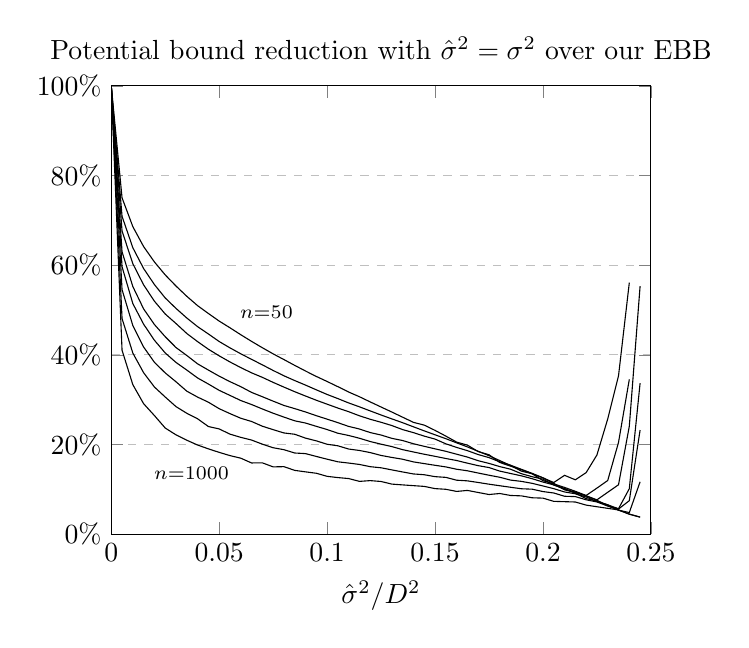
\begin{tikzpicture}
	\begin{axis}[
		title={Potential bound reduction with $\hat{\sigma}^2 = \sigma^2$ over our EBB},
		xlabel={$\hat{\sigma}^2/D^2$},
		xmin=0, xmax=0.25,
		ymin=0, ymax=100,
		xtick={0,0.05,0.1,0.15,0.2,0.25},
		ytick={0,20,40,60,80,100},
		yticklabel=$\pgfmathprintnumber{\tick}\%$,
		legend pos=south west,
		ymajorgrids=true,
		grid style=dashed,
		xticklabel style={/pgf/number format/fixed},
	]
	\addplot[] coordinates {
(0.0, 100.0)(0.005, 75.02420135527589)(0.01, 68.58202038924931)(0.015, 64.13237924865832)(0.02, 60.71118820468343)(0.025, 57.819103972950124)(0.03, 55.33498759305211)(0.035, 53.04630381803412)(0.04, 50.96)(0.045, 49.21383647798742)(0.05, 47.51937984496124)(0.055, 46.02446483180428)(0.06, 44.47806354009077)(0.065, 42.99625468164794)(0.07, 41.57386785449146)(0.075, 40.20618556701031)(0.08, 38.93352812271731)(0.085, 37.63596809282088)(0.09, 36.38328530259366)(0.095, 35.17191977077364)(0.1, 34.04558404558404)(0.105, 32.88447909284196)(0.11, 31.68666196189132)(0.115, 30.639494026704146)(0.12, 29.481792717086833)(0.125, 28.35195530726257)(0.13, 27.228412256267408)(0.135, 26.0778859527121)(0.14, 24.930555555555557)(0.145, 24.31129476584022)(0.15, 23.140495867768596)(0.155, 21.862068965517242)(0.16, 20.525224602626125)(0.165, 19.8489010989011)(0.17, 18.413793103448278)(0.175, 17.707618393960193)(0.18, 15.975103734439834)(0.185, 15.161957270847692)(0.19, 14.36426116838488)(0.195, 13.452299245024022)(0.2, 12.542837559972584)(0.205, 11.51473612063057)(0.21, 13.115845539280958)(0.215, 12.117177097203728)(0.22, 13.71280724450194)(0.225, 17.65424557116677)(0.23, 25.69558101472995)(0.235, 35.30794546309356)(0.24, 56.085994309200125)
		}node[pos=0.4](endofplotsquare){} ;
	\node [above right] at (endofplotsquare) {$\scriptstyle n=50$};
	\addplot[] coordinates {
(0.0, 100.0)(0.005, 70.89337175792507)(0.01, 63.881401617250674)(0.015, 59.23076923076923)(0.02, 55.66502463054187)(0.025, 52.67538644470868)(0.03, 50.345622119815665)(0.035, 48.20627802690583)(0.04, 46.2800875273523)(0.045, 44.646680942184155)(0.05, 42.96218487394958)(0.055, 41.54639175257732)(0.06, 40.22289766970618)(0.065, 38.983050847457626)(0.07, 37.75811209439528)(0.075, 36.50485436893204)(0.08, 35.31669865642994)(0.085, 34.25047438330171)(0.09, 33.23943661971831)(0.095, 32.18604651162791)(0.1, 31.152073732718893)(0.105, 30.228310502283104)(0.11, 29.257246376811594)(0.115, 28.39173405211141)(0.12, 27.475468331846567)(0.125, 26.572187776793623)(0.13, 25.704225352112676)(0.135, 24.84689413823272)(0.14, 23.93385552654482)(0.145, 23.03030303030303)(0.15, 22.155172413793103)(0.155, 21.28755364806867)(0.16, 20.35928143712575)(0.165, 19.453924914675767)(0.17, 18.46808510638298)(0.175, 17.502124044180118)(0.18, 16.397621070518266)(0.185, 15.306122448979592)(0.19, 14.054514480408859)(0.195, 13.463166807790008)(0.2, 11.925042589437819)(0.205, 11.205432937181664)(0.21, 10.414902624894157)(0.215, 9.551986475063398)(0.22, 8.622147083685546)(0.225, 10.262725779967159)(0.23, 11.961722488038278)(0.235, 20.45616535994298)(0.24, 34.51481696687972)
		}node[pos=0.693](endofplotsquare){} ;
	%\node [above] at (endofplotsquare) {$\scriptstyle n=75$};
	\addplot[] coordinates {
(0.0, 100.0)(0.005, 67.61904761904762)(0.01, 60.31468531468531)(0.015, 55.5921052631579)(0.02, 51.95618153364632)(0.025, 49.0990990990991)(0.03, 46.97406340057637)(0.035, 44.75524475524475)(0.04, 42.93478260869565)(0.045, 41.246684350132625)(0.05, 39.766839378238345)(0.055, 38.40304182509506)(0.06, 37.142857142857146)(0.065, 35.97560975609756)(0.07, 34.97005988023952)(0.075, 33.844339622641506)(0.08, 32.7906976744186)(0.085, 31.76605504587156)(0.09, 30.804077010192525)(0.095, 29.86577181208054)(0.1, 28.98230088495575)(0.105, 28.11816192560175)(0.11, 27.302275189599133)(0.115, 26.394849785407725)(0.12, 25.61105207226355)(0.125, 24.94736842105263)(0.13, 24.217118997912316)(0.135, 23.316062176165804)(0.14, 22.633744855967077)(0.145, 21.859039836567927)(0.15, 21.196754563894523)(0.155, 20.141700404858298)(0.16, 19.335347432024168)(0.165, 18.61861861861862)(0.17, 17.74675972083749)(0.175, 17.063492063492063)(0.18, 16.12265084075173)(0.185, 15.369458128078819)(0.19, 14.454277286135694)(0.195, 13.555992141453832)(0.2, 12.561334641805692)(0.205, 11.307767944936087)(0.21, 9.881422924901186)(0.215, 9.251968503937007)(0.22, 8.537782139352306)(0.225, 7.647058823529412)(0.23, 9.333333333333334)(0.235, 11.00832562442183)(0.24, 24.0625)(0.245, 55.32786885245902)
		}node[pos=1.0](endofplotsquare){} ;
	%\node [above] at (endofplotsquare) {$n=100$};
	\addplot[] coordinates {
(0.0, 100.0)(0.005, 62.98342541436464)(0.01, 55.223880597014926)(0.015, 50.23041474654378)(0.02, 46.753246753246756)(0.025, 44.03292181069959)(0.03, 41.61735700197239)(0.035, 39.84819734345351)(0.04, 37.981651376146786)(0.045, 36.58969804618117)(0.05, 35.233160621761655)(0.055, 34.00673400673401)(0.06, 32.89473684210526)(0.065, 31.612903225806452)(0.07, 30.647709320695103)(0.075, 29.658385093167702)(0.08, 28.702290076335878)(0.085, 27.994011976047904)(0.09, 27.245949926362297)(0.095, 26.41509433962264)(0.1, 25.644699140401148)(0.105, 24.858757062146893)(0.11, 24.022346368715084)(0.115, 23.448275862068964)(0.12, 22.646657571623464)(0.125, 22.10242587601078)(0.13, 21.36181575433912)(0.135, 20.871862615587848)(0.14, 20.157068062827225)(0.145, 19.58495460440986)(0.15, 19.02313624678663)(0.155, 18.471337579617835)(0.16, 17.825537294563844)(0.165, 17.189460476787954)(0.17, 16.375)(0.175, 15.77639751552795)(0.18, 15.061728395061728)(0.185, 14.478527607361963)(0.19, 13.480392156862745)(0.195, 12.804878048780488)(0.2, 12.257281553398059)(0.205, 10.94890510948905)(0.21, 10.194174757281553)(0.215, 9.101941747572816)(0.22, 7.907542579075426)(0.225, 7.38498789346247)(0.23, 6.521739130434782)(0.235, 5.669481302774427)(0.24, 10.136674259681094)(0.245, 33.693843594009984)
		}node[pos=1.0](endofplotsquare){} ;
	%\node [above] at (endofplotsquare) {$n=150$};
	\addplot[] coordinates {
(0.0, 100.0)(0.005, 59.642857142857146)(0.01, 51.41955835962145)(0.015, 46.820809248554916)(0.02, 43.24324324324324)(0.025, 40.40920716112532)(0.03, 38.292682926829265)(0.035, 36.5967365967366)(0.04, 34.831460674157306)(0.045, 33.47826086956522)(0.05, 32.06751054852321)(0.055, 30.942622950819672)(0.06, 29.8)(0.065, 28.90625)(0.07, 27.915869980879542)(0.075, 26.96629213483146)(0.08, 26.102941176470587)(0.085, 25.270758122743683)(0.09, 24.778761061946902)(0.095, 24.041811846689896)(0.1, 23.32761578044597)(0.105, 22.504230118443317)(0.11, 22.0)(0.115, 21.38157894736842)(0.12, 20.650406504065042)(0.125, 20.064205457463885)(0.13, 19.523809523809526)(0.135, 18.838304552590266)(0.14, 18.322981366459626)(0.145, 17.81874039938556)(0.15, 17.35159817351598)(0.155, 16.867469879518072)(0.16, 16.417910447761194)(0.165, 15.828402366863905)(0.17, 15.27165932452276)(0.175, 14.847161572052402)(0.18, 14.057971014492754)(0.185, 13.525179856115107)(0.19, 13.0)(0.195, 12.357954545454545)(0.2, 11.614730878186968)(0.205, 10.985915492957746)(0.21, 10.0)(0.215, 9.396914446002805)(0.22, 8.531468531468532)(0.225, 7.5524475524475525)(0.23, 6.3113604488078545)(0.235, 5.594405594405594)(0.24, 7.462686567164179)(0.245, 23.214285714285715)
		}node[pos=1.0](endofplotsquare){} ;
	%\node [above] at (endofplotsquare) {$n=200$};
	\addplot[] coordinates {
(0.0, 100.0)(0.005, 54.54545454545455)(0.01, 46.52173913043478)(0.015, 41.732283464566926)(0.02, 38.32116788321168)(0.025, 35.95890410958904)(0.03, 33.980582524271846)(0.035, 31.888544891640866)(0.04, 30.56379821958457)(0.045, 29.428571428571427)(0.05, 27.977839335180054)(0.055, 26.881720430107528)(0.06, 25.848563968668408)(0.065, 25.126903553299492)(0.07, 24.069478908188586)(0.075, 23.300970873786408)(0.08, 22.565320665083135)(0.085, 22.273781902552205)(0.09, 21.4123006833713)(0.095, 20.80536912751678)(0.1, 20.044052863436125)(0.105, 19.696969696969695)(0.11, 18.976545842217483)(0.115, 18.658280922431867)(0.12, 18.181818181818183)(0.125, 17.551020408163264)(0.13, 17.10261569416499)(0.135, 16.69980119284294)(0.14, 16.110019646365423)(0.145, 15.728155339805825)(0.15, 15.355086372360844)(0.155, 14.990512333965844)(0.16, 14.473684210526315)(0.165, 14.12639405204461)(0.17, 13.627992633517495)(0.175, 13.138686131386862)(0.18, 12.681159420289855)(0.185, 12.050359712230216)(0.19, 11.764705882352942)(0.195, 11.327433628318584)(0.2, 10.73943661971831)(0.205, 10.13986013986014)(0.21, 9.40766550522648)(0.215, 8.996539792387543)(0.22, 8.290155440414507)(0.225, 7.253886010362694)(0.23, 6.540447504302926)(0.235, 5.344827586206897)(0.24, 4.810996563573883)(0.245, 11.67192429022082)
		}node[pos=1.0](endofplotsquare){} ;
	%\node [above] at (endofplotsquare) {$n=300$};
	\addplot[] coordinates {
(0.0, 100.0)(0.005, 48.091603053435115)(0.01, 40.38461538461539)(0.015, 36.0)(0.02, 32.8125)(0.025, 30.58252427184466)(0.03, 28.440366972477065)(0.035, 26.956521739130434)(0.04, 25.726141078838175)(0.045, 24.0)(0.05, 23.46153846153846)(0.055, 22.304832713754646)(0.06, 21.58273381294964)(0.065, 20.97902097902098)(0.07, 20.068027210884352)(0.075, 19.269102990033222)(0.08, 18.83116883116883)(0.085, 18.095238095238095)(0.09, 17.956656346749227)(0.095, 17.325227963525837)(0.1, 16.71641791044776)(0.105, 16.129032258064516)(0.11, 15.85014409221902)(0.115, 15.536723163841808)(0.12, 15.041782729805014)(0.125, 14.794520547945206)(0.13, 14.324324324324325)(0.135, 13.866666666666667)(0.14, 13.421052631578947)(0.145, 13.246753246753247)(0.15, 12.820512820512821)(0.155, 12.658227848101266)(0.16, 12.030075187969924)(0.165, 11.881188118811881)(0.17, 11.519607843137255)(0.175, 11.138014527845037)(0.18, 10.79136690647482)(0.185, 10.451306413301662)(0.19, 10.117647058823529)(0.195, 10.023310023310023)(0.2, 9.49074074074074)(0.205, 9.174311926605505)(0.21, 8.447488584474886)(0.215, 8.371040723981901)(0.22, 7.657657657657658)(0.225, 7.174887892376682)(0.23, 6.263982102908278)(0.235, 5.369127516778524)(0.24, 4.464285714285714)(0.245, 3.7861915367483294)
		}node[pos=1.0](endofplotsquare){} ;
	%\node [above] at (endofplotsquare) {$n=500$};
	\addplot[] coordinates {
(0.0, 100.0)(0.005, 41.02564102564103)(0.01, 33.333333333333336)(0.015, 29.09090909090909)(0.02, 26.446280991735538)(0.025, 23.66412213740458)(0.03, 22.142857142857142)(0.035, 20.945945945945947)(0.04, 19.871794871794872)(0.045, 19.01840490797546)(0.05, 18.235294117647058)(0.055, 17.51412429378531)(0.06, 16.939890710382514)(0.065, 15.873015873015873)(0.07, 15.897435897435898)(0.075, 15.0)(0.08, 15.048543689320388)(0.085, 14.218009478672986)(0.09, 13.88888888888889)(0.095, 13.574660633484163)(0.1, 12.88888888888889)(0.105, 12.608695652173912)(0.11, 12.393162393162394)(0.115, 11.764705882352942)(0.12, 11.934156378600823)(0.125, 11.740890688259109)(0.13, 11.155378486055778)(0.135, 10.980392156862745)(0.14, 10.81081081081081)(0.145, 10.64638783269962)(0.15, 10.150375939849624)(0.155, 10.0)(0.16, 9.523809523809524)(0.165, 9.747292418772563)(0.17, 9.285714285714286)(0.175, 8.8339222614841)(0.18, 9.059233449477352)(0.185, 8.620689655172415)(0.19, 8.532423208191126)(0.195, 8.108108108108109)(0.2, 8.02675585284281)(0.205, 7.308970099667774)(0.21, 7.2368421052631575)(0.215, 7.166123778501628)(0.22, 6.472491909385114)(0.225, 6.109324758842444)(0.23, 5.7507987220447285)(0.235, 5.396825396825397)(0.24, 4.444444444444445)(0.245, 3.7974683544303796)
		}node[pos=0.85](endofplotsquare){} ;
	\node [below left] at (endofplotsquare) {$\scriptstyle n=1000$};
	\end{axis}
	\end{tikzpicture}
	\vspace{-10pt}
	\caption[The percent reduction our EBB could yet achieve]{The percent reduction in the 0.5 probability bound that going from our EBB to using Bennett's inequality (perfect variance information, $\hat{\sigma}^2 = \sigma^2$) achieves, for $n=50,75,100,150,200,300,500,1000$.}
	\label{biggraph4}
\end{figure}



Secondly, a comparison is made of the further improvement in confidence over our EBB that might be achieved with perfect information about the variance; specifically that, Bennett's inequality is used assuming $\hat{\sigma}^2=\sigma^2$. 
This improvement is plotted in Figure \ref{biggraph4}, which shows that when the variance is small, uncertainty about the variance is the most detrimental to an EBB, such as ours.
However, in general, going from our EBB to perfect variance information shrinks the bounds by about another third.

In this way (although the results are loose) we can witness that our EBB provides approximately a half-way mark from existing state-of-the-art EBBs to an impossible ideal of having perfect variance information.

The purpose of developing a novel EBB was to see if it could be used to improve the selection of samples in the context of stratified sampling (particularly of the Shapley Value).
The performance of this new EBB offers (against others) in the context of choosing samples for stratified Stratified Sampling is considered in Section \ref{section:statistics_results}.


%Within this context, finite-sample \textit{concentration inequalities} are used to place bounds on 
%the variation of sample statistics around their population values.
%Such bounds are applied in a range of data science contexts for a variety of prediction, machine learning and hypothesis testing tasks, including:
%change detection \cite{KiferShaiGehrke2004,8000571} 
%and classification \cite{Zia-UrRehman2012} in data streams;
%outlier analysis in large databases \cite{Aggarwal2015};
%online optimisation \cite{FlaxmanKalaiMcMahan2005,AgarwalDekelXiao2010}; and, of most relevance to this paper, 
%online prediction and learning problems \cite{Cesa-BianchiLugosi2006,%Maron1997,
%Mnih:2008:EBS:1390156.1390241,DBLP:conf/aaai/ThomasTG15,Maurer50empiricalbernstein},
%particularly in settings with \textit{bandit feedback} \cite{AuerCesa-BianchiEtal_SIAM2003,AudibertBubeck_COLT2009,Tran-ThanhChapmanRJ_AAAI2009}. 
% Bandit feedback describes settings where a decision-maker wishes to learn about a system, and to do this, chooses samples from a set of actions and receives feedback regarding their chosen actions only, in the form of a realization of a random variable. 
%Specifically, the decision-maker does not see how the system would have responded, if they had chosen a different action.
%



For the ease of this application of our EBB we hand-tuned a function approximating our EBB's numerical probability 0.5 bound,
The process of creating the expression involved plotting the numerical data, and manually fitting an approximate symbolic expression:
\begin{equation}\label{eq:prob_bound} \p\left(\mu-\hat{\mu}\ge \frac{D}{\sqrt{n}}\; \min\left[ \sqrt{2\log 2},
\footnotesize
\left(\begin{matrix*}[c]
\frac{3}{5}\sqrt{\min\left[1,\frac{\hat{\sigma}^2}{D^2}+\frac{25}{n}\right]} \\+ \ln\left(\max\left[1,n\left(1-\frac{\hat{\sigma}^2}{D^2}\right)\right]\right)^{-4}\end{matrix*}
\normalsize
\right)\right]\right) 
\lessapprox 0.5 \end{equation}




\subsection{Stratified sampling via EBBs and sequential unions}\label{section:unionising_ebbs}

To create a bound for the error of our stratified mean estimator from EBBs we need to use probability unions to bind them together:

\begin{theorem}\label{triangle_theorem1}
If we have $m$ strata of sizes $N_i$. If we have taken $n_i$ samples $X_{i,1},X_{i,2},\dots,X_{i,n_i}$ from each stratum, resulting in a stratum sample mean $\hat{\mu}_i = \frac{1}{n_i}\sum_{j=1}^{n_i}X_{i,j}$ and stratum sample variance $\hat{\sigma}_i^2=\frac{1}{n_i}\sum_{j=1}^{n_i}(X_{i,j}-\hat{\mu}_i)^2 $.
If the error in the sample mean of a stratum is bounded by an Empirical Bernstein Bound:
$\quad \p(\hat{\mu}_i-\mu_i \ge Z(n_i,D_i,\hat{\sigma}^2_i,t)) \le t $\\
Then the error in our stratified estimation is probability bounded:
$$ \p\left(\hat{\mu}-\mu \ge \sum_{i=1}^m\frac{N_i}{\sum_kN_k} Z(n_i,D_i,\hat{\sigma}^2_i,t/m)\right)\le t $$
\end{theorem}
\begin{proof}
We begin by considering that the stratified mean estimate is given by:
$$ \hat{\mu} = \sum_{i=1}^m\frac{N_i}{\sum_kN_k} \hat{\mu}_i ~~~~~~~\text{and thus:}~~~~~~~ \hat{\mu}-\mu = \sum_{i=1}^m\frac{N_i}{\sum_kN_k} (\hat{\mu}_i-\mu_i)$$
Thence because we can scale (by positive factor) the inside of the EBB inequality (for any $j\in\{1,\dots, m\}$):
\begin{equation}\label{equation_partial_union1} \p\left(\frac{N_j}{\sum_kN_k}(\hat{\mu}_j-\mu_j) \ge \frac{N_j}{\sum_kN_k}Z(n_j,D_j,\hat{\sigma}^2_j,t)\right) \le t \end{equation}
adding identical terms to both sides of the inner inequality gives:
\begin{equation}\label{equation_partial_union2} \p\left(\sum_{i=1}^m\frac{N_i}{\sum_kN_k}(\hat{\mu}_i-\mu_i) \ge \frac{N_i}{\sum_kN_k}Z(n_k,D_k,\hat{\sigma}^2_k,t) + \sum_{\substack{i=1 \\ i\ne j}}^m\frac{N_i}{\sum_kN_k}(\hat{\mu}_i-\mu_i)\right) \le t \end{equation}
now since equation \ref{equation_partial_union1} also holds for any $l\in\{1,\dots, m\}$ other $j$ then:
$$ \p\left(\frac{N_l}{\sum_kN_k}(\hat{\mu}_l-\mu_l) \ge \frac{N_l}{\sum_kN_k}Z(n_l,D_l,\hat{\sigma}^2_l,t)\right) \le t $$
hence by adding terms to both sides of the inner inequality:
\begin{equation}\label{equation_partial_union3} \p\left(\begin{matrix*}\frac{N_i}{\sum_kN_k}Z(n_k,D_k,\hat{\sigma}^2_k,t)\\ + \sum_{\substack{i=1 \\ i\ne j}}^m\frac{N_i}{\sum_kN_k}(\hat{\mu}_i-\mu_i)\end{matrix*} \ge \begin{matrix*} \frac{N_i}{\sum_kN_k}Z(n_k,D_k,\hat{\sigma}^2_k,t) +\\ \frac{N_l}{\sum_kN_k}Z(n_l,D_l,\hat{\sigma}^2_l,t) +\\ \sum_{\substack{i=1 \\ i\ne j\\i\ne l}}^m\frac{N_i}{\sum_kN_k}(\hat{\mu}_i-\mu_i)\end{matrix*}\right) \le t \end{equation}
Applying probability union (lemma \ref{prob_union}) to equations \ref{equation_partial_union2} and \ref{equation_partial_union3} gives:
$$ \p\left(\hat{\mu}-\mu \ge \begin{matrix*} \frac{N_i}{\sum_kN_k}Z(n_k,D_k,\hat{\sigma}^2_k,t) +\\ \frac{N_l}{\sum_kN_k}Z(n_l,D_l,\hat{\sigma}^2_l,t) +\\ \sum_{\substack{i=1 \\ i\ne j\\i\ne l}}^m\frac{N_i}{\sum_kN_k}(\hat{\mu}_i-\mu_i)\end{matrix*}\right) \le 2t $$
Repeating this process of taking equation \ref{equation_partial_union1} for a new index, adding appropriate terms to the inner inequality and using probability union lemma \ref{prob_union}, ultimately gives:
$$ \p\left(\hat{\mu}-\mu \ge \sum_{i=1}^m\frac{N_i}{\sum_kN_k} Z(n_i,D_i,\hat{\sigma}^2_i,t)\right)\le mt $$
And scaling $t$ gives result.
\end{proof}

The result of this proof is an inequality bounding the error of the stratified mean estimate by the number of samples and the width and sample variance of each of the strata - which is exactly what we are looking for.
We can apply this theorem with our choice of EBB to create a bound for the stratified mean error, which we can then seek to minimise.

What is worth noting is that this process of binding EBBs together by a series of probability unions is expected to result in a rather weak bound, as probability unions are not very strong.
And that this weakness is expected to increase with larger numbers of strata (ie. larger $m$) as there are more probability unions needed to bind it together.

If we are concerned about the absolute error of the stratified estimate $|\hat{\mu}-\mu|$ then we can conduct a similar procedure, and utilize the triangle inequality - as done by \cite{2013arXiv1306.4265M}.

\begin{theorem}\label{triangle_theorem2}
In exactly the same context as theorem \ref{triangle_theorem1}, that:
$$ \p\left(|\hat{\mu}-\mu| \ge \sum_{i=1}^m\frac{N_i}{\sum_kN_k} Z(n_i,D_i,\hat{\sigma}^2_i,t/2m)\right)\le t $$
\end{theorem}
\begin{proof}
If $ \p(\hat{\mu}_i-\mu_i \ge Z(n_i,D_i,\hat{\sigma}^2_i,t)) \le t$ then
$ \p(|\hat{\mu}_i-\mu_i| \ge Z(n_i,D_i,\hat{\sigma}^2_i,t)) \le 2t$.\\
Then by repeated application of probability unions (similar to that process used in the proof of theorem \ref{triangle_theorem1}) we get:
\begin{equation}\label{partial_equation_part11} \p\left(\sum_{i=1}^m\frac{N_i}{\sum_kN_k} |\hat{\mu}_i-\mu_i| \ge \sum_{i=1}^m\frac{N_i}{\sum_kN_k} Z(n_i,D_i,\hat{\sigma}^2_i,t) \right) \le 2mt \end{equation}
Now, via the triangle inequality:
$$\hat{\mu}-\mu = \sum_{i=1}^m\frac{N_i}{\sum_kN_k} (\hat{\mu}_i-\mu_i) ~~~~~~~~~~\text{implies}~~~~~~~~~~ |\hat{\mu}-\mu| \le \sum_{i=1}^m\frac{N_i}{\sum_kN_k} |\hat{\mu}_i-\mu_i| $$
then $ \p(|\hat{\mu}-\mu| > \sum_{i=1}^m\frac{N_i}{\sum_kN_k}|\hat{\mu}_i-\mu_i|) \le 0 $ and by probability union with \eqref{partial_equation_part11}:
$$ \p\left(|\hat{\mu}-\mu| \ge \sum_{i=1}^m\frac{N_i}{\sum_kN_k} Z(n_i,D_i,\hat{\sigma}^2_i,t)\right)\le 2mt $$
And the result follows by scaling $t$.
\end{proof}

We give this second theorem in addition to the first make clear, that sampling to minimise either the error, or the absolute error essentially amounts to minimising the same target in this context.
And also to illustrate exactly how weak probability unions are.

The triangle equality $|A+B|\le |A|+|B|$, is only an equality in the event that the elements $A$ and $B$ are of the same sign, and in the context of theorems \ref{triangle_theorem1} and \ref{triangle_theorem2} we are effectively developing a bound assuming all the errors of the estimates of the strata are additive - which is positively the worst case.
Whereas we know that (or can possibly assume) that the errors in the strata estimates are actually independent of each other, and hence a overestimation in one stratum estimate is likely to be somewhat countered by an underestimation in another.
Using this knowledge, stronger bounds are very possible - and we explore and develop this in the following Section \ref{section:SEBB}.


